\chapter{Specifications}
\label{chap:specifications}
\setstretch{1.5}
\section{Purpose}
\label{sec:purpose}
The purpose of this project, consisting of preliminary studies and bachelor thesis, is to add an additional layer of safety to collaborative robotic systems, which should detect and avoid collisions.
Currently most systems use force and torque sensors which are telling the robot to stop its motion, as soon as a collision occurs. This presumes a given amount of force or torque to lead the robot to an action. In term of the collaboration between human and machine, this principle fits the given needs. But when it comes to lighter objects like containers with (sometimes toxic) liquids or other unstable objects, the robot will not stop its motion because the sensor did not get a measurement within the specified force range.
Systems with force sensors, only react when a certain force threshold is reached. Collisions with light objects may not reach the force threshold and therefor may not stop the robot motion. To avoid such cases, a vision system shall monitor the workspace and detect objects, then adapt the robots trajectories according to the position of obstacles to avoid a collision.

\section{Description and goals}
\label{sec:description}

The main goal is to integrate a vision system to detect any unexpected temporary objects in real-time in a robot workspace to add an extra layer of safety for the employee and to reduce downtime within the production process. The work shall be performed in a collaboration with the local department of Bern University of Applied Science for architecture, wood and civil engineering, AHB in Biel, using their Fanuc CR35iA Cobot. 
The CR35iA is currently the biggest collaborative robot available on the market. It has a maximum payload of 35kg and a reach of 1813mm. The robot is placed in a factory like building, surrounded with other robots and machines, therefore representing an industrial environment, similar to the foreseen use in the industry.
The detection of obstacles inside the robots workspace shall be realized by using 3D sensors. The data provided by these sensors will be processed by the GPU-Voxels Algorithm into voxelized maps. Two maps shall be implemented, one for the workspace and one for the robot model and its trajectories. Using the robots joint speeds, trajectories may be predicted to a certain point and can be integrated into the robot model map. By comparing the maps with each other, upcoming collisions can be predicted. Upon detecting collisions, the robot trajectories shall be adapted to avoid the previously predicted collision, without stopping the robots motion to calculate an alternative route for the robots motion. For extra credit, the system shall be demonstrated in a dynamic workspace, with human detection integrated.
The Bern University of Applied Science executes multiple Bachelor Theses in robotics, and specifically for collaborative tasks, a group of students working in this field has been build. Teamwork is highly required and recommended to avoid making the same mistakes and to be sure to share knowledge and progress. Tasks which can be shared or even adapted offer a great advantage to all students in this group. In addition, it helps the experts to coordinate the work which is done. 


\section{System Specifications}
\label{sec:requirements}
Based on the content in section \ref{sec:description}, Description and goals, a system specification has been elaborated by the author. 

\subsection{System Functions}
\subsubsection{Object detection}
The System shall detect Objects inside the robot workspace using one or more stereo cameras.
Possible cameras are the Microsoft Kinect and the Asus Xtion ProLite, which are available at BFH TI for this Thesis. A third possible camera would be the e-con Systems Tara or TaraXL, which would have to be ordered. These cameras would also be available for users in the industry as they are available on the market. The cameras shall provide point cloud data which will be processed using the GPU-Voxels algorithm. The algorithm provides functionality regarding voxelisation, data compression and map generation.

\subsubsection{Motion Planning}
When an obstacle is identified within the workspace of the robot, the algorithm should compare its position with the planned trajectories of the robot. If an upcoming collision is identified according to the obstacles position, a new trajectory shall be calculated, so that the robot can move to its goal without colliding with the obstacle.

The Open Motion Planner Library (OMPL) should provide different planning algorithms, which could be used to solve the motion planning. New ways, avoiding the obstacle, shall be calculated by using the voxel map which the system provides. The system shall calculate the shortest way form the robots current position to its goal by using the free spaces which the map provides.

\subsubsection{Robot Communication}
The used Fanuc CR35iA Cobot only runs Karel code. Karel is a programming language based on Pascal. To use any C++ library for the motion planning, a communication between the robot using Karel and the C++ program needs to be implemented. For this case, Fanuc enables socket communication over TCP/IP, which can be used to transfer robot pose and joint speeds to the C++ code. The C++ Code processes the data from the robot and the object detection and delivers desired go-to positions which will be read by the Karel code and used to move the robot to the goal.

\subsection{Safety and perfomance requirements}
\subsubsection{Jam avoidance}
\label{subsec:jamavoid}
Between the two joints of Fanuc CR35iA Cobot, marked in Figure 2.1 no force measurement is available, which means objects or human limbs can be jammed between the joints. This is a massive safety risk for the user of the robot. To increase the safety of the user, any detected object in between the joints should lead to an immediate stop of the robot movement which would lead to a jam. If possible, the robot shall turn and move away from the object to prohibit a jam and again calculate a different path to its initial goal without damaging anyone or anything and without pausing the production.

\begin{figure}[h]
	\begin{center}
		\centering
		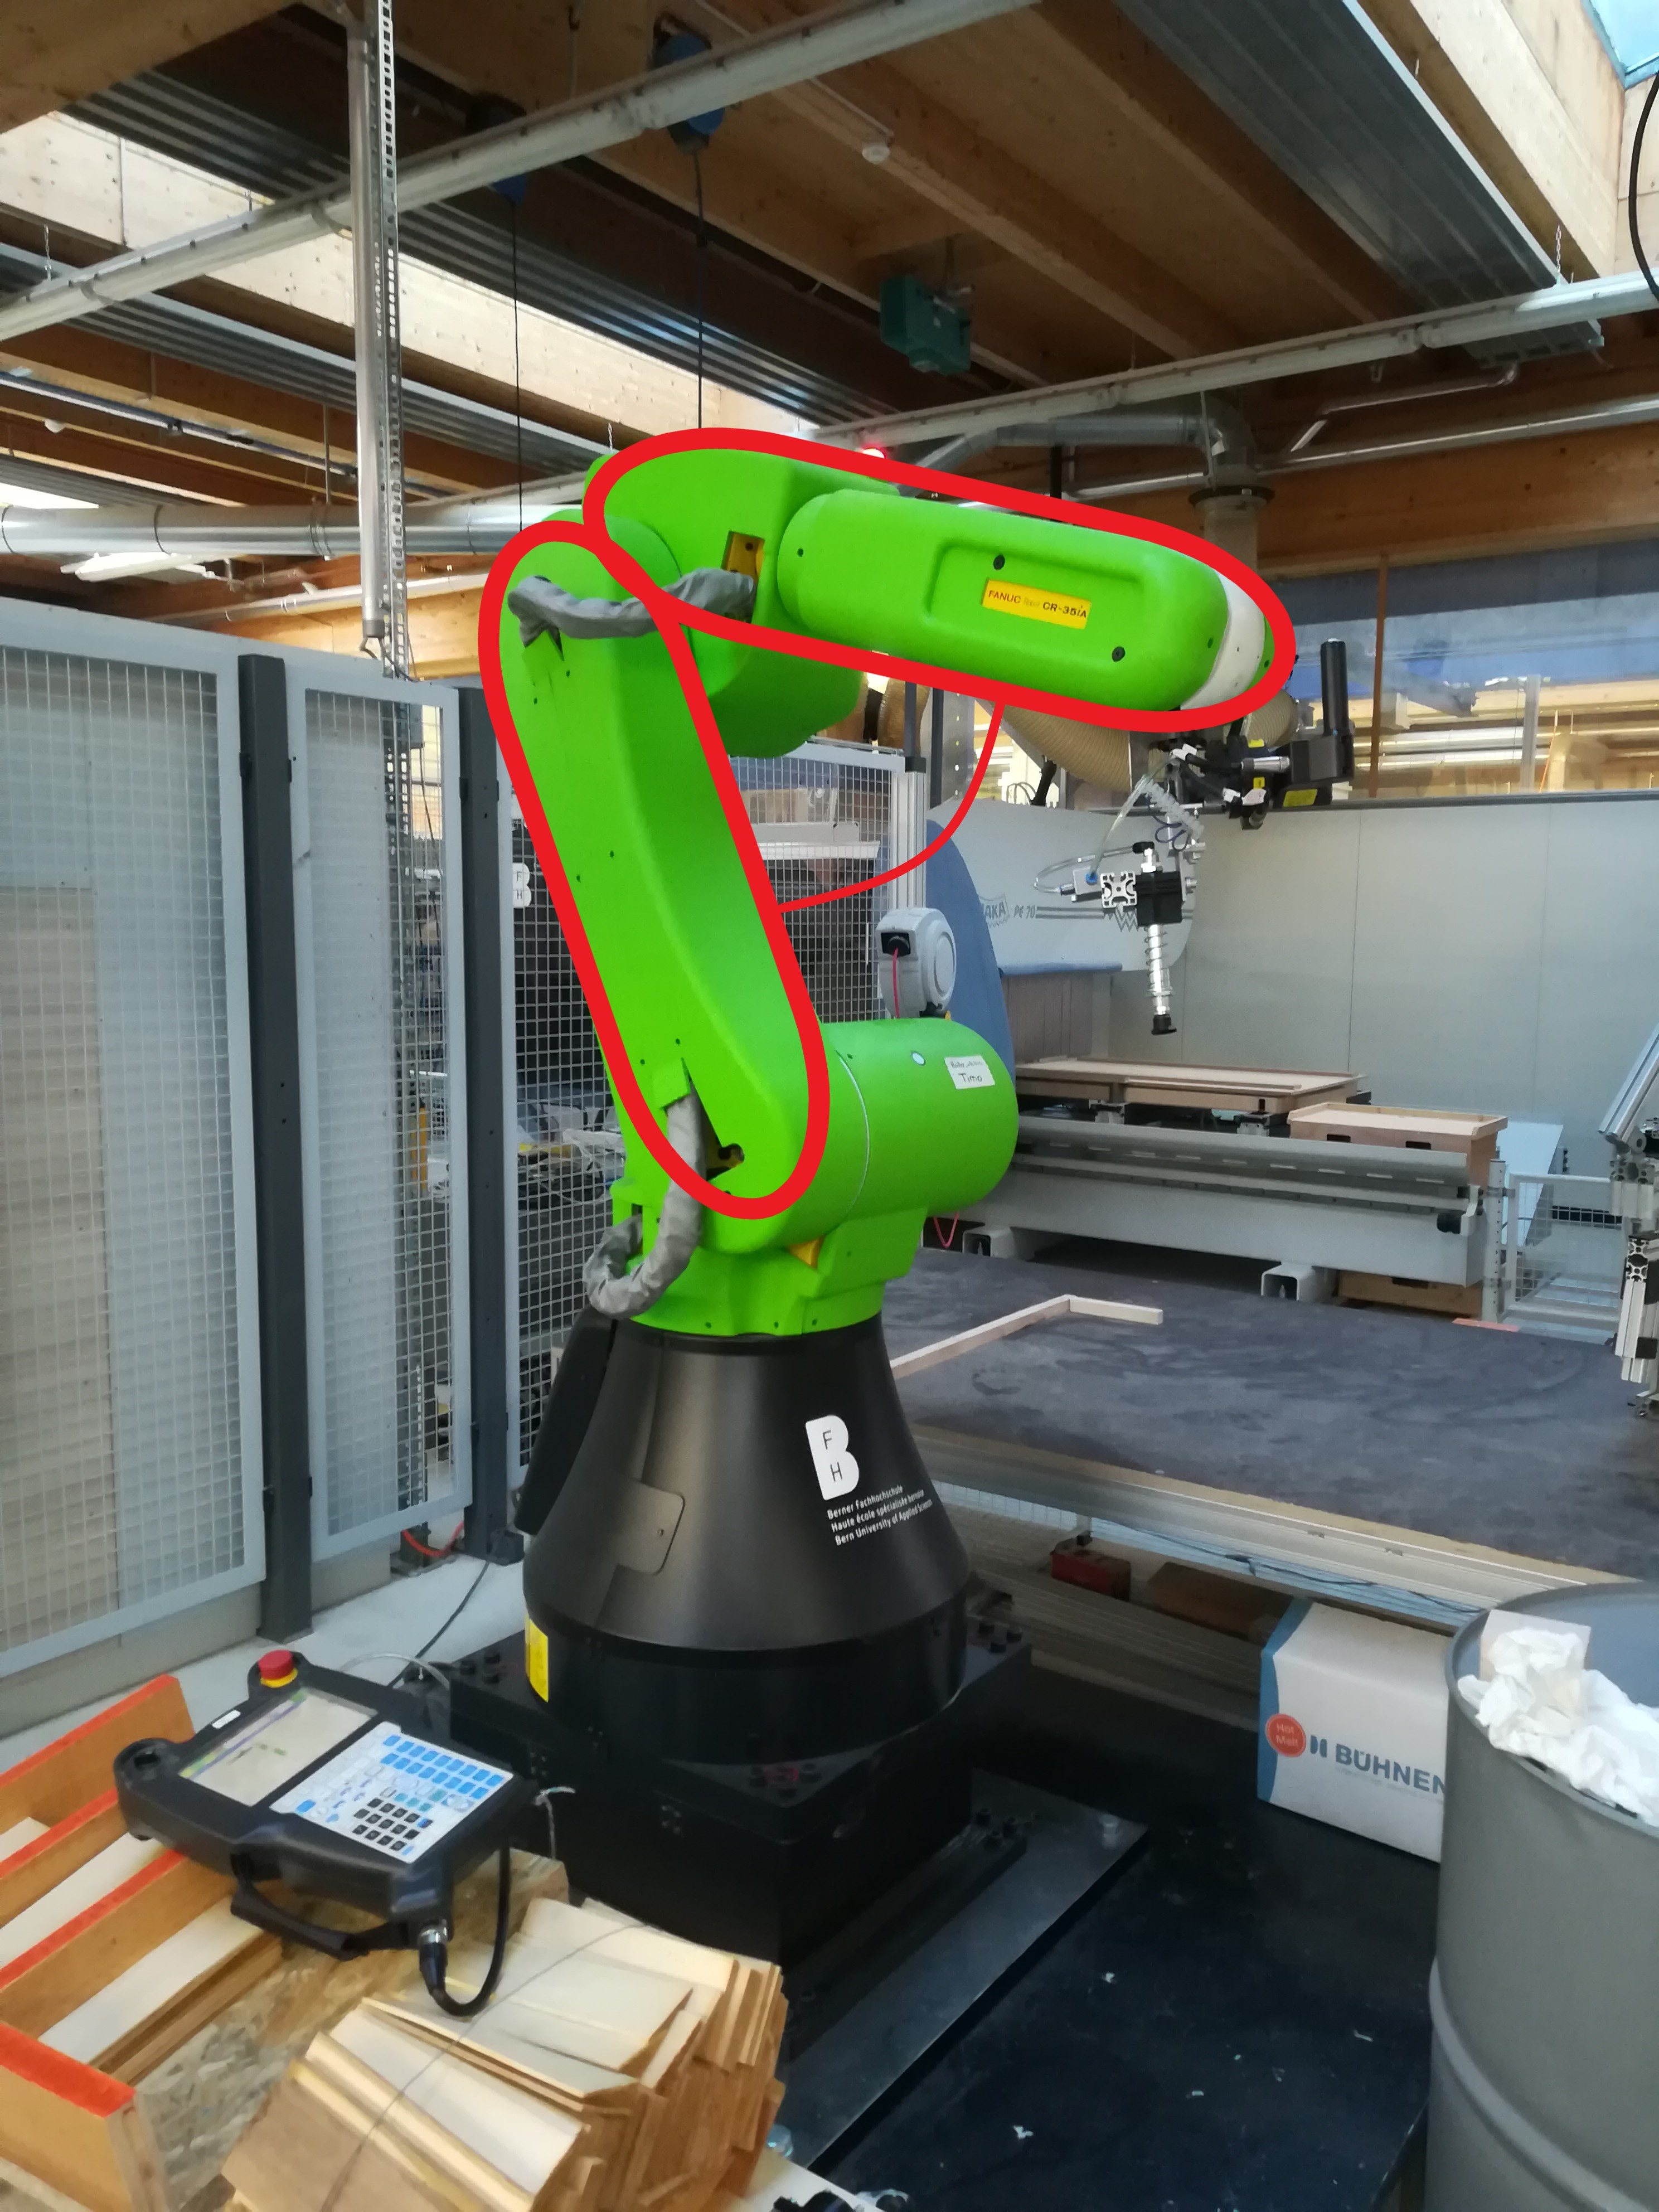
\includegraphics[width=0.40\linewidth]{images/fanuc_joint.jpg}
		\caption{Fanuc CR35iA Cobot at BFH AHB}
		\label{fig:fanucrob}
	\end{center}
\end{figure}

\subsubsection{Safety stop}
\label{subsec:safetystop}
When a certain minimum distance to the obstacle is reached, the robot should perform an immediate stop for safety reasons. 
This minimal distance can be defined by the user of the system, considering the speed and given circumstances in the workspace.

If the goal is not reachable, due to any object preventing a collision free movement (e.g. a bottle laying on the goal position), the robot shall stop until the obstacle is removed and the goal is free.

\subsubsection{Environment}
Regarding the current environment of the robot and future use, the system should work in a normal industrial environment, without being too sensitive to changes of the light conditions depending on the time of day. Therefor additional light sources may be included while testing the system.


\newpage
\section{System Flow Chart}
\label{sec:flow chart}
\begin{figure}[!ht]
	\centering
	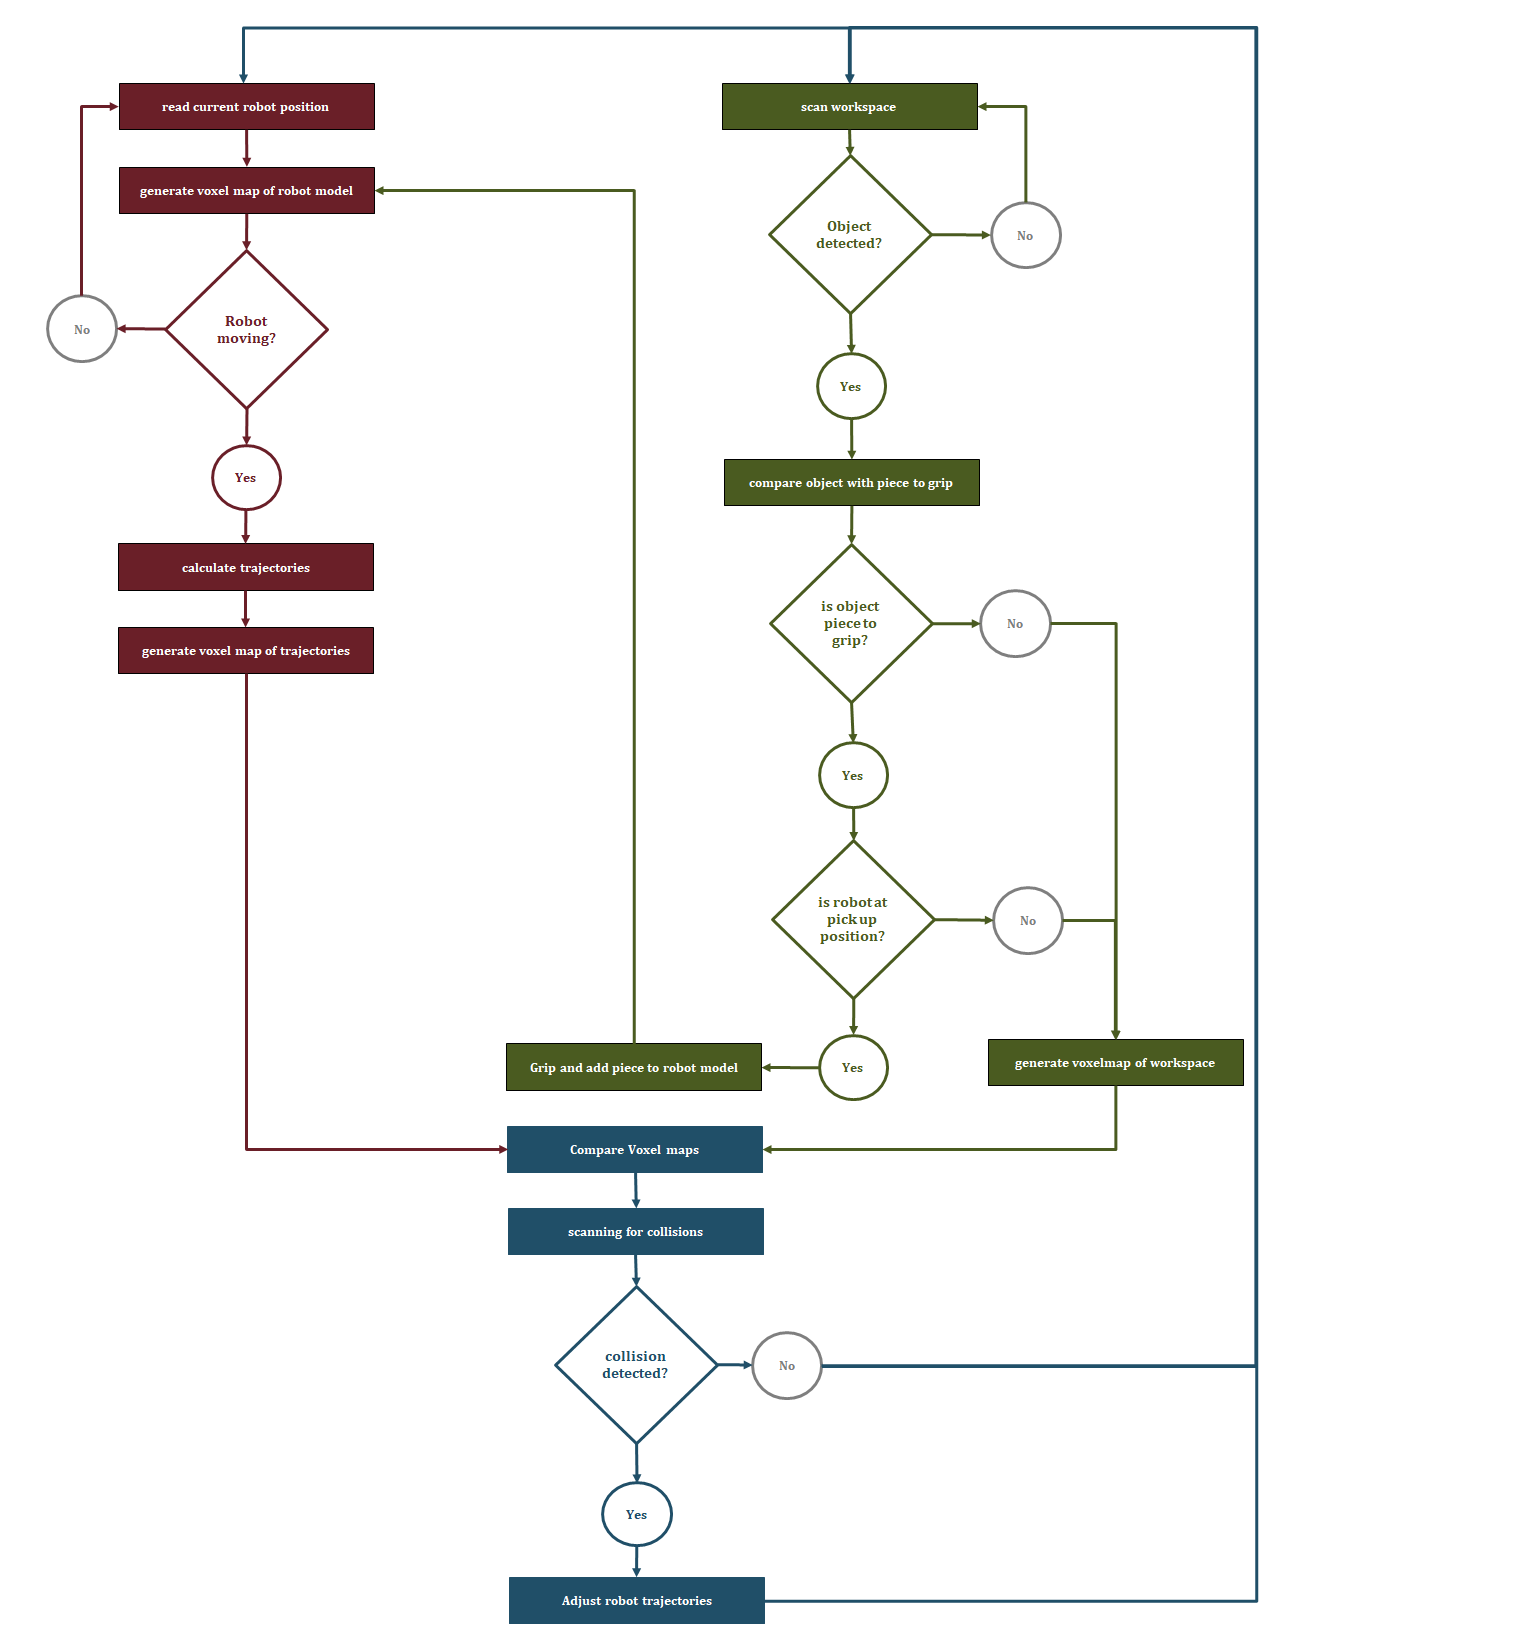
\includegraphics[width=1.2\linewidth]{images/flowchart}
	\caption{Block diagram of the System }
	\label{fig:bd1}
\end{figure}

\newpage
%Based on the maximum speed of 250mm/s of the CR35iA a scanning frequency of 4Hz has been defined as a default value for a static workspace. 


%The system shall be implemented on a Fanuc CR35iA robot, currently the biggest collaborative robot on the market. The robot is used with a Fanuc R-30iB copntroller.
%
%To achieve the goal of this project, the system task may be divided into the following subtasks, which will be explained further in this chapter:
%\begin{itemize}
%	\item Communicating with the robot
%	\item Detect objects
%	\item Path planning
%\end{itemize}
%
%\subsection{Communicating with the robot}


